\documentclass{article}

% \usepackage{blindtext}
\usepackage[english]{babel}
\usepackage[utf8]{inputenc}
\usepackage{geometry}  % set the margins to (_)in on all sides
\usepackage{graphicx}              % to include figures
\usepackage{amsmath}               % great math stuff
\usepackage{amssymb}
\usepackage{amsfonts}              % for blackboard bold, etc
\usepackage{amsthm}                % better theorem environments
%\usepackage{xcolor}
\usepackage{cite}
\usepackage{cancel}
\usepackage{bm}
\usepackage{enumitem}
% \usepackage{enumerate,multicol}

% fonts
\usepackage[T1]{fontenc}
\usepackage{lmodern}                         % enhanced computer modern
% \usepackage{concmath}                        % computer modern concrete
 % \usepackage{times}                      % times new roman
 % \usepackage{newtx}               % math times new roman - new version
% \usepackage{garamondx}                       % garamond expert
% \usepackage[garamondx,cmbraces]{newtxmath}     % garamond expert + NewTX Math
% \usepackage{url}
\usepackage{hyperref}
% \hypersetup{
%     colorlinks,
%     linkcolor={blue!80!black},
%     citecolor={green!80!black},
%     urlcolor={cyan!80!black},
%     filecolor=magenta,
%     linkbordercolor={blue!80!black},
%     citebordercolor={blue!100!black},
%     urlbordercolor={cyan!80!black},
%     filebordercolor={magenta!80!black},
%     hyperfootnotes=true,
% }
 
% \urlstyle{same}
\usepackage{tikz}

% various theorems, numbered by section

\newtheorem{thm}{Theorem}[section]
\newtheorem{lem}{Lemma}[section]
\newtheorem{prop}{Proposition}[section]
\newtheorem{cor}{Corollary}[thm]
\newtheorem{conj}{Conjecture}[section]
\theoremstyle{remark}
\newtheorem{rem}{Remark}[section]
\theoremstyle{definition}
\newtheorem{dft}{Definition}[section]

\DeclareMathOperator{\id}{id}

\newcommand{\bd}[1]{\mathbf{#1}}  % for bolding symbols
\newcommand{\RR}{\mathbb{R}}      % for Real numbers
\newcommand{\QQ}{\mathbb{Q}}      % for Integers
\newcommand{\ZZ}{\mathbb{Z}}      % for Integers
\newcommand{\NN}{\mathbb{Z}^+}      % for Naturals
\newcommand{\FF}{\mathbb{F}}      % for Fields
\newcommand{\col}[1]{\left[\begin{matrix} #1 \end{matrix} \right]}
\newcommand{\comb}[2]{\binom{#1^2 + #2^2}{#1+#2}}

% \setlength{\parindent}{0cm}
\setlength{\parskip}{0.25cm}

\begin{document}


\title{Remarks on Loopring: Draft}
\author{Supersymmetry\\
        \texttt{da447m@yahoo.com}}

\date{}
\maketitle
%\nocite{*}

\begin{abstract}
The purpose of this document is to provide an easy to understand explanation of the ideas behind the mathematics in Loopring's White Paper, having in mind those with no background in the subject. It requires only high school math. I'm not part of the Loopring organization, this paper reflects only my personal analysis.
\end{abstract}

% \tableofcontents
% \clearpage

\section{The anatomy of a trade}\label{sect:sect1}

Every order has two basic elements: two assets offered for trading and an exchange rate. The price is the exchange rate with one of the assets fixed as parameter. Lets assume that Alice and Bob want to trade their tokens A and B. Alice has 15 tokens A and she wants 4 tokens B for them, Bob has 10 tokens B and he wants 30 tokens A for them.

Who is buying and who is selling? This depends only on the asset we fix to give price quotations. If the token A is the reference, then Alice is buying tokens B for $\frac{15}{4}=3.75$ XTA, while Bob is selling 10 tokens B for $\frac{30}{10}=3.00$ XTA. In the case of fixing token B as reference we say that Alice is selling 15 tokens A for $\frac{4}{15}=0.26666667$ XTB and Bob is buying 10 tokens A for $\frac{10}{30}=0.33333334$ XTB. Hence, who's the buyer or seller is purely arbitrary.

In the first situation Alice is willing to pay a higher price than the price Bob is selling his tokens for, in the second situation Bob is willing to pay a higher price than the price Alice is selling her tokens for. It is clear that \emph{a trade is possible whenever the buyer is willing to pay an equal or higher price than the selling price}, no matter how we fix the prices. If we recall our basic arithmetic we learned in school we verify easily that

$$
\displaystyle\frac{\frac{15}{4}}{\frac{30}{10}}=\frac{3.75}{3.00}=\frac{0.33333334}{0.26666667}=\frac{\frac{10}{30}}{\frac{4}{15}}=\frac{15}{4}\cdot\frac{10}{30}=\frac{150}{120}=1.25>1.
$$

These trivial observations allow for a somewhat powerful generalization: to decide if a set of $n$ orders is to be filled, in total or partially\footnote{In the example given it is clear that Bob won't be able to get 30 Tokens A since Alice is offering only 15. The condition to perform a trade does not guarantee a complete filling of the order, but that the desired price will be kept.}, \emph{observing a price equal or small to the intended price}, all we need to know is the product of each one of the exchange rates \emph{as buy orders}. If this product results in a number greater or equal to 1, all the $n$ orders can be either partially, or totally filled.

Another way of saying it is this: for each order, the exchange rate is represented by a fraction such that the numerator is the amount of tokens getting out $\overrightarrow{x}$ and the denominator the amount of tokens getting in $\underleftarrow{y}$

$$\dfrac{\overrightarrow{x}}{\underleftarrow{y}},$$
%
so the product is equal to one if everybody is giving exactly what their counterparts want, and it is greater if somebody is giving more. We will henceforth write the fractions representing exchange rates always in this fashion.

To illustrate, in the example above Alice's intended trade is to give 15 tokens A and receive 4 tokens B, Bob's is to give 10 tokens B and receive 30 tokens A. Since $\frac{15}{4}\cdot\frac{10}{30}\geq 1$ they will trade observing a price equal to, or smaller than the intended price of each one of them. In the former case a discount can be given, what will be seen ahead.

\subsection{Proof of the conditions to perform a trade}\label{sect:subsect1}

First, we remark that for each order with a given token getting out we need a counterpart order where this same token is getting in, otherwise there is no possible trade for that token. Furthermore, with such proviso, we also remark that even if the counterpart order involves a third token, what matters for a given token $T$ is simply having $\overrightarrow{x}T$ and $\underleftarrow{y}T$ at any given fraction representing an exchange rate.

To see this, suppose that now we have Alice, Bob and Charlie, so that Alice wants to give $x_1$ tokens A and receive $y_1$ tokens B, Bob wants to give $x_2$ tokens B and receive $y_2$ tokens C, and Charlie wants to give $x_3$ tokens C and receive $y_3$ tokens A. We have the counterparts and the trade is possible if, and only if,
$$
\frac{x_1\cdot x_2\cdot x_3}{y_1\cdot y_2\cdot y_3}\geq1.
$$
%
Before we prove this for the general case, we need to make an observation. If there is more than one buy order involving the same pairs, we need to group these orders as a single order. For instance, suppose we have the three buy orders
$$
\frac{1A}{2B},\quad\frac{1A}{3B},\quad\frac{5B}{2A}.
$$
%
If we simply multiply them, the result is $\frac{5}{12}<1$, but still clearly the trades can be made at the exchange rates proposed. In such cases we group the orders alike and we end up at the result
$$
\frac{1A+1A}{2B+3B}\cdot\frac{5B}{2A}=\frac{2A}{5B}\cdot\frac{5B}{2A}=1,
$$
what shows that the orders can be filled.

We now consider the general case. Let's assume all orders involving the same pairs are grouped as a single order. Let's assume that for each order where there are $x_i$ tokens $T_i$ getting out, there is at least one order where $y_j$ units of the same token $T_i$ is getting in. We end up with the following $n$ orders $O$: $O_1=\frac{x_1T_1}{y_1T_2}, O_2=\frac{x_2T_2}{y_2T_3},\cdots, O_n=\frac{x_nT_n}{y_nT_1}$.

This means that all the $n$ orders $O$ form a closed ring of orders, connected as in the figure below:

\begin{center} 
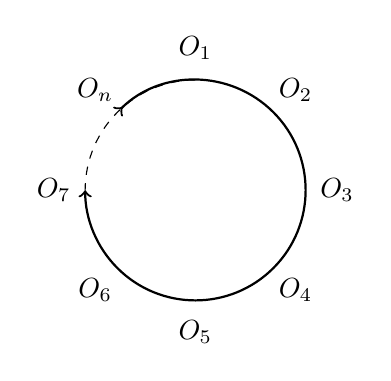
\begin{tikzpicture}[scale=2]
    %
    % Independent parameters
    \pgfmathsetmacro\dth{360/8}                            % angular increment
    \def\angleOffset{135}                                    % starting angle
    \def\dialR{0.7}                                           % dial radius
    \def\dialLabelOffset{.2}                                % label radial offset
    %
    % Dependent parameters
    % \pgfmathsetmacro\angleTip{-10.5*\dth+\angleOffset}      % tip angle
    \pgfmathsetmacro\dialLabelR{\dialR+\dialLabelOffset}    % label radius
    %   
    % draw arc
    \draw[thick,>->]
        (\angleOffset:\dialR) arc (\angleOffset:-180:\dialR);
  
    \draw[dashed]
        (90:\dialR) arc (90:180:\dialR);
    %
    % write labels
    \foreach
    [
        var=\k,
        var=\dialLabel,
        evaluate=\k as \th using -\k*\dth+\angleOffset,
    ]
    in {0/$O_n$,1/$O_1$,2/$O_2$,3/$O_3$,4/$O_4$,5/$O_5$,6/$O_6$,7/$O_7$}%
    { 
     \draw (\th:\dialLabelR) node {\dialLabel};
    }
\end{tikzpicture}
\end{center}
%
When we have a closed ring of orders we call it a match-ring, and we can evaluate whether all trades can be at least partially filled or not.

Lets represent the amount of tokens $T$ actually traded by $\#T$\footnote{Recall that the orders might be only partially filled.}; this is the amount observing a price equal to, or smaller than, the intended price for all parties involved. This means that a buy order $O_i=\frac{x_iT_i}{y_iT_{i+1}}$ intends to give away $x_i$ tokens $T_i$ and to receive $\#T_{i+1}\geq y_i$ tokens $T_{i+1}$, or to give away $\#T_{i}\leq x_i$ tokens $T_i$ and to receive $y_i$ tokens $T_{i+1}$ -- or a combination of both. Hence
$$
\frac{\#T_{i}}{\#T_{i+1}}\leq\frac{x_i}{y_i}\Longrightarrow\frac{x_i}{y_i}\cdot\#T_{i+1}\geq\#T_{i}
$$
%
Let $\prod_n$ be the product of all $n$ orders, it is very easy to verify that
$$
\frac{x_1}{y_1}\cdot\frac{x_2}{y_2}\cdot...\cdot\frac{x_n}{y_n}\cancel{\#T_{1}}\cdot\cancel{\#T_{2}}\cdot...\cdot\cancel{\#T_{n}}\geq\cancel{\#T_{1}}\cdot\cancel{\#T_{2}}\cdot...\cdot\cancel{\#T_{n}}
$$
$$
\prod_n=\frac{x_1}{y_1}\cdot\frac{x_2}{y_2}\cdot...\cdot\frac{x_n}{y_n}\geq1
$$
Therefore, in a match-ring, where all parties involved get the best exchange rates possible, the product of all $n$ orders is necessarily equal to, or greater than, 1.

\subsection{Basics of discounts and fees}\label{sect:subsect2}

Once we have a match-ring, a discount is applicable to all trades equally if, and only if, $\prod_n>1$. Notice that if $\prod_n>1$, then $\prod_n=1+\alpha\Longrightarrow\prod_n\cdot\frac{1}{1+\alpha}=1$, so $\frac{1}{1+\alpha}$ is the total discount that can be distributed to each of the $n$ orders. In other words: it is the product of $1-\gamma$ $n$ times, where $\gamma$ is the discount equally applicable to each one of the $n$ orders $O$, thus $\frac{1}{1+\alpha}=(1-\gamma)^n$. This leads to
$$
\gamma=1-\frac{1}{\sqrt[\leftroot{-2}\uproot{2}n]{\prod_n}}.
$$
Let me explain what was done: since we have $\prod_n>1$, this means that $\prod_n$ has to be equal to some number greater than 1, so this number can be written as 1 plus some real number $\alpha>0$. Then, with some little algebra we get $\frac{1}{1+\alpha}$, this is a number smaller than 1 which represents how much "excess" can be cut off of $\prod_n$ and still we will have all orders filled. For instance, if $\frac{1}{1+\alpha}=0.9$ this means that 10\% of $\prod_n$ can be given back.

This ``excess'' can be distributed equally to each of the $n$ orders as a fixed discount $\gamma$. This is because when $\prod_n=1$, all orders are executed exactly at their exchange rates. Why is that? Because in this case the amounts getting in and out of the same tokens are exactly the same, so their ratio is 1, so the product of their ratios is 1.

If $\prod_n>1$, this means that at least in one case someone paid a higher price than the one the counterpart was asking for, so the counterpart got the discount that could have been shared. Now, to treat all orders in the ring-match with equanimity, we distribute that discount to all of them. 

Let's recall our first example to see how this can be done. Alice has 15 tokens A and she wants 4 tokens B for them, Bob has 10 tokens B and he wants 30 tokens A for them. If the token A is the reference, then Alice is buying tokens B for $\frac{15}{4}=3.75$ XTA, while Bob is selling 10 tokens B for $\frac{30}{10}=3.00$ XTA. If we execute the orders making Alice pay $3.75$ XTA, Bob has advantage. Bob sells 4 tokens B for $3.75$ XTA, so he receives 15 Tokens A, this satisfies Alice's order entirely, but Bob was supposed to get only 12 executing the order using his exchange rate -- $3.00$ XTA. 

Let's calculate the discount: $\frac{150}{120}=1.25$, so $\frac{1}{1.25}=0.8=(1-\gamma)^2$, thus the exchange rate that makes things even is $\sqrt{0.8}\cdot 3.75\approx 3.35410197$ XTA. Bob gives 4 tokens B and receives 13.41640786 tokens A, more than the 12 he was expecting for those 4 tokens. Alice receives 4 tokens B as intended but gives only 13.41640786 tokens A in exchange, less than the 15 she was willing to give for those 4 tokens.

In this same situation (where $\prod_n>1$), it is possible for the ring miners to get fees, a part of the costs savings or some combination of both. In this case, a discount can still be offered also to the users, making the deal advantageous to all parties by using the market making properties of the match-ring and increased turn-over and liquidity.

% \subsection{Open rings closure}\label{sect:subsect3}

% Suppose we have Alice and Bob with orders $\frac{1A}{2B},\frac{2B}{3C}$. We need Charlie to come up with $\frac{xC}{1A}$, $x\geq3$, to close the ring.

% \section{Ring miner ranking}\label{sect:sect2}

\end{document}
